\label{CADZeichnung}

Wie schon im Kapitel \ref{Entwurf} beschrieben wurde, war es für uns als Gruppe von größter Wichtigkeit, unsere gesammelten Konzepte in die Gehäuseentwicklung einfließen zu lassen, um so, die ideale Bauform für unser Messgerät zu entwickeln und zu fertigen. \\
Für die Erstellung der Zeichnung in einem CAD Programm haben einerseits die einfache Anpassungsfähigkeit, die drei Dimensionale Visualisierung des Gehäuses und die Zeichnungsdatei als Quelldatei für den 3D-Druck gesprochen.\\
Das Gehäuse wurde in zwei Teile aufgeteilt. Zum einen der Deckel, aus Abbildung \ref{fig:Zeichnung_Deckel}, in welchem das \ac{LCD}-Display, die einzelnen Taster für die Auswahl der Menüpunkte und die \ac{LED}s für die Visualisierung der Luftqualität integriert sind. \\
Zum anderen das Gehäuse, welches in Abbildung \ref{fig:Zeichnung_Schale} dargestellt wird. Hier ist das Arduino Modul, das PIN-Breadboard, der Mikro-SD-Karten-Adapter und der C0$_2$-Sensor platziert. An dieser Stelle war es wichtig, dass der Sensor außerhalb des Gehäuses platziert wird, damit die Richtigkeit der resultierenden Messergebnisse sichergestellt ist. Der Arduino selbst wurde am Gehäuserand platziert, damit ein einfacher Zugang zu den externen Ausgängen gewährleistet ist. So muss nicht bei jeder neuen Softwareversion das gesamte Gehäuse geöffnet werden.

\begin{figure}[!hbt]
	\centering
	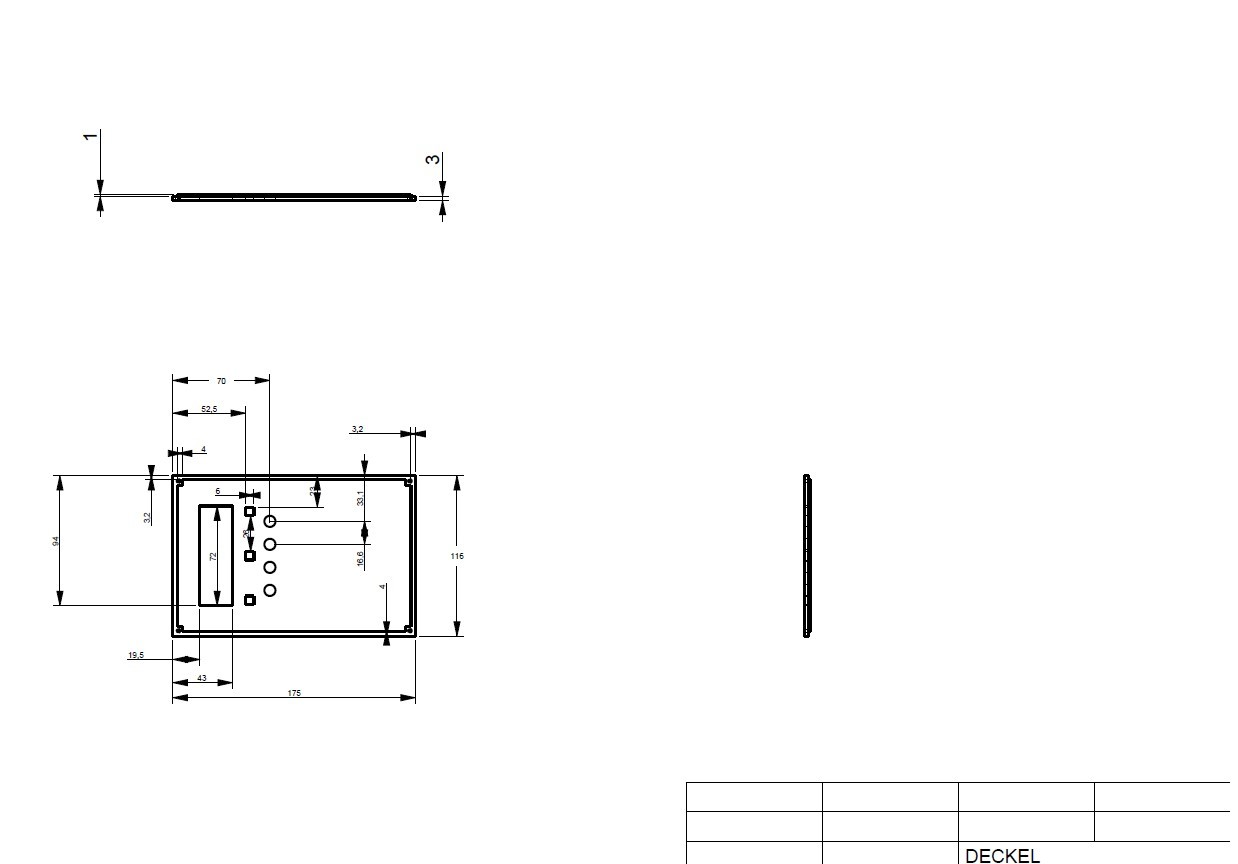
\includegraphics[width=0.9\linewidth]{Images/CAD-Deckel}
	\footnotesize \\Quelle: eigene Zeichnung
	\caption{CAD-Zeichnung für den Deckel des Gehäuses}
	\label{fig:Zeichnung_Deckel}
\end{figure}

\begin{figure}[!hbt]
	\centering
	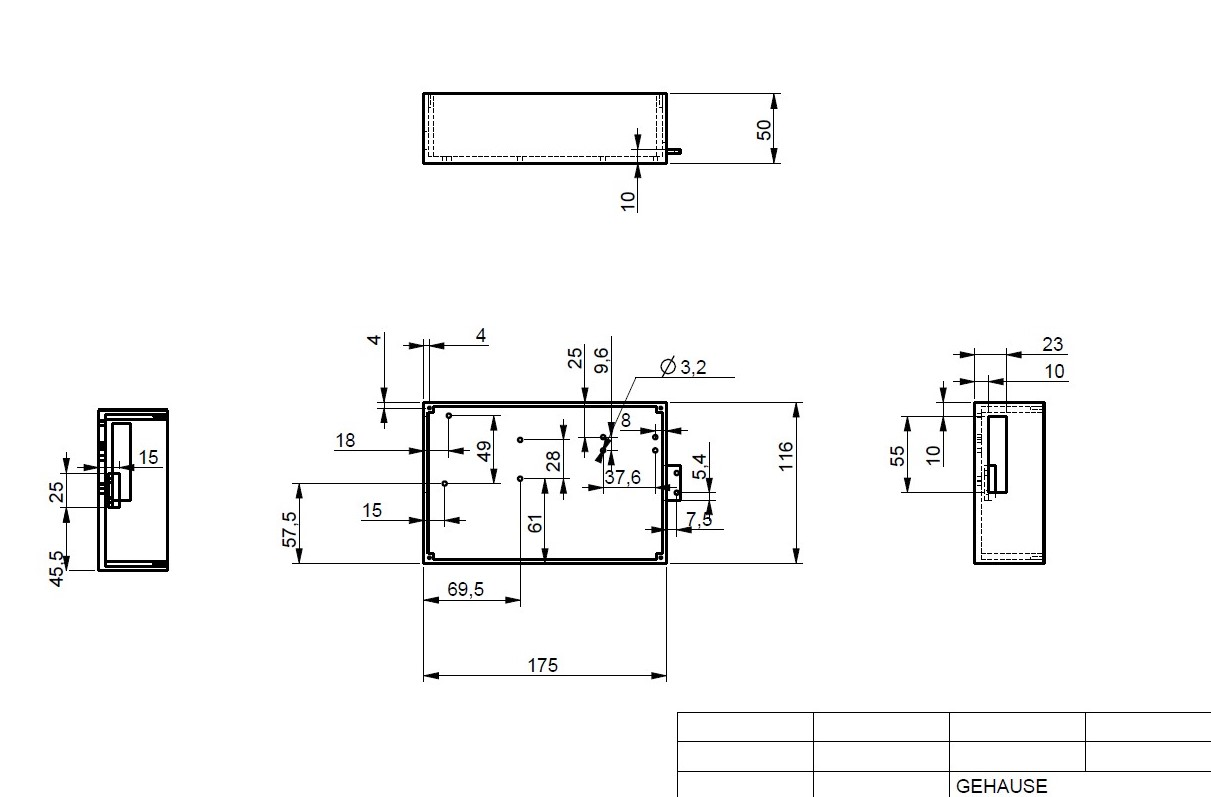
\includegraphics[width=0.9\linewidth]{Images/CAD-Schale}
	\footnotesize \\Quelle: eigene Zeichnung
	\caption{CAD-Zeichnung für die Schale des Gehäuses}
	\label{fig:Zeichnung_Schale}
\end{figure}

